\section{Annotation Generation}\label{SecAnnotGen}

Given a security property encoded as an MVA, the annotation generation
procedure generates JML-annotations that capture this property,
\emph{i.e.}, the program does not violate the generated annotations
if and only if it respects the encoded property.
% security property encoded by the MVA.
As explained above, the procedure is defined in several steps:
\begin{inparaenum}[(\itshape i\upshape)]
\item the monitor is completed; %(as described in Section~\ref{SecMVA});
\item the annotations are generated at the method specification level,
as special set-annotations; and
\item the method specification-level set-annotations are inlined in
the method body.
%\item the special \CaseJML construct that is used to make the
%annotations more compact is translated into a sequence of \Set
%annotations.
\end{inparaenum}
%Notice that the order of the last two steps can be swapped.
Notice that the special \CaseJML statement could be translated into
standard JML annotations as well.

For each step we prove that the old and the new program are bisimilar,
\emph{i.e.}, we show for every translation step
\(\alpha\) there exists a relation \(R\) such that:
\[{\small
\begin{array}{l}
\forall b, \sigma_1, \sigma_2, \tau_1, v_1.
\etp{P}{b,\sigma_1}{v_1, \sigma_2} \wedge
R(\sigma_1, \tau_1) \Rightarrow \\
\qquad
\exists \tau_2, v_2.
\etp{\alpha(P)}{b, \tau_1}{v_2, \tau_2} \wedge
R(\sigma_2, \tau_2)
\end{array}}
\]
and vice versa. Additionally, we show that the initial program states
are related by \(R\), and from this we can conclude that for any
reachable state of the monitored program, there exists a related state,
reachable in the translated program.

\marginnote{This is specific of the second step, not general.}
A natural way to prove this is by induction over the derivation length.
To be able to apply induction, we typically require that the body \(b\) does
not contain new variables. However, the translation introduces new (ghost)
variables to encode the MVA, at specific points in the program. For
these points, separate preservation lemmas have to be proven.
Further, to be able to complete the proof, we need to ensure that in both
bodies the same branches of conditional expressions and statements are
taken, and that the same values get assigned to the store. Therefore,
we prove a stronger result, adding that also the values  %resulting values
\(v_1\) and \(v_2\) are the same (however, sometimes this holds only
under certain conditions).

%% Commented to save space
% This section presents more details of the different translation steps,
% and presents the relation that witnesses the bisimulation.  Further,
% we discuss the special conditions under which the bisimulation holds.

%\begin{figure}
%\begin{center}
%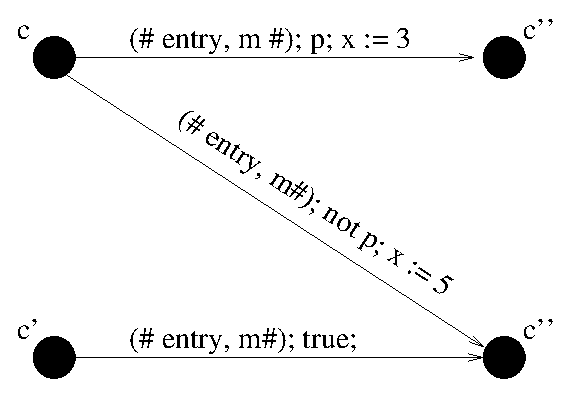
\epsfig{file=annotgen_example, width=4cm}
%\end{center}
%\caption{MVA fragment to illustrate set-annotation
%generation}\label{FigAnnotGenExample}

%\end{figure}

\paragraph{Completion of the automaton}
The first translation step does not change the program itself, it only
completes the MVA. Suppose that \(P\) is a monitored program, where
\(\mva(P)\) is deterministic and wellformed. Then the translation to a
monitored program with a total MVA, \(\alpha_1(P)\), is defined as:
% This is complete_MP in MonitoredProgramCompletessRelation
\[{\small
\alpha_1(P) = \opri \mva := \complete(P.\mva), \program := P.\program
\clri
}
\]

The relation that is preserved between executions of \(P\) and
%% This is monitor_related_states
\marginnote{Should we add the condition on ghost variables?}
\(\alpha_1(P)\) is the following (where \(\sigma\) is a state of
\(P\) and \(\tau\) is a state of \(\alpha_1(P)\)):
\[{\small
R(\sigma, \tau) =\\
 \begin{array}[t]{l}
  (\pif {\sigma.\stuck}{\tau.\mvastate.\cp = \halted\\\ }
        {\sigma.\mvastate.\cp = \tau.\mvastate.\cp}) \:\wedge
  \neg \tau.\stuck \:\wedge\\
  (\sigma.\mvastate.\stA = \tau.\mvastate.\stA) \:\wedge
  (\sigma.\progstate = \tau.\progstate)
\end{array}}
\]

To prove that this relation is preserved for any body \(b\), we make
use of equivalence (\ref{MVAcompletionProp}) on
Page~\pageref{MVAcompletionProp} and we observe further that
\begin{inparaenum}[(\itshape i\upshape)]
\item if \stuck has been set, it remains set,
\item if the MVA is total and \halted is reached, it is never left, and
\item if the MVA is total, \stuck is never set.
\end{inparaenum} Formally, where \(P\) is a monitored program, and
\(Q\) is a monitored program with total MVA:
\[{\small
\begin{array}[t]{rl}
\sigma_1.\stuck \wedge \etp{P}{b,\sigma_1}{v,\sigma_2} \Rightarrow &
\sigma_2.\stuck \\
\sigma_1.\mvastate.\cp = \halted \wedge
\etp{Q}{b,\sigma_1}{v,\sigma_2} \Rightarrow &
\sigma_2.\mvastate.\cp = \halted \\
\neg \sigma_1.\stuck \wedge \etp{Q}{b,\sigma_1}{v,\sigma_2} \Rightarrow &
\neg \sigma_2.\stuck
\end{array}}
\]

%% Rephrased
% For our running example, applying translation \(\alpha_1\) means that
% where class \texttt{Messaging} as shown above was first monitored
% with the partial MVA in Figure~\ref{FigExample}, after the translation
% it is monitored with the total MVA in Figure~\ref{FigCompleteMVA}.
For our running example, applying the translation \(\alpha_1\) means that
the class \texttt{Messaging} instead of being monitored by the partial MVA
in Figure~\ref{FigExample}, it is monitored by the total MVA in
Figure~\ref{FigCompleteMVA}.
% TODO AT: for some reason I get Fig 2 here instead of Fig 3.


\paragraph{From MVA to Annotations}

\begin{figure}[t]
\[{\small
\begin{array}{rcl}
\alpha_2(P) & = &\opri \classes :=
\{\alpha_{2, \mathcal{C}}(c, P.\mva) \mid c \in P.\program.\classes\} \clri\\

\alpha_{2,\mathcal{C}}(c, a) & = &
\mathsf{if\ }c.\name \not = a.\clname \mathsf{\ then\ }c\\
&&
\mathsf{else\ }c \:\opri
 \begin{array}[t]{l}
 \gvs := c.\gvs \cup \newgvs(a)\\
 \inv := \Conj(\Not(\Eq(\texttt{cp}, \texttt{halted})), c.\inv)\\
 \methods := \{\alpha_{2,\mathcal{M}}(m, a) \mid m \in c.\methods\} \clri
\end{array}\\
\alpha_{2,\mathcal{M}}(m, a) & = & m \: \opri
  \begin{array}[t]{l}
  \preset := \begin{array}[t]{l}
             m.\preset; \alpha_{2,\mathcal{E}}(\entry, m.\name, a);
             \Assert(\Not(\Eq(\texttt{cp}, \texttt{halted}))),
             \end{array}\\
  \postset := m.\postset; \alpha_{2, \mathcal{E}}(\exit, m.\name, a)\\
  \excset := m.\excset; \alpha_{2, \mathcal{E}}(\excexit, m.\name, a)
  \clri
  \end{array}\\
\alpha_{2, \mathcal{E}}(e, n, a) & = &
  \alpha_{2, \mathcal{T}}(\{t \mid t \in a.\trans \wedge
                                   t.\event = \opri \event := e,
                                                    \mname := m \clri
                           \})\\
\alpha_{2, \mathcal{T}}(ts) & = &
  \CaseJML(
    \{(\begin{array}[t]{l}
       \Eq(\texttt{cp}, \texttt{q}),\\
       \CaseJML(\{(t.\guard, \Set(\texttt{cp}, t.\tcp; t.\action)) \mid
                  t \in ts \wedge t.\scp = \texttt{q}
               \}))\\
    \mid \texttt{q} \in a.\cps
    \})
    \end{array}
\end{array}}
\]
\caption{Formal definition of translation MVA into annotations}
\label{FigMVAtoAnnot}
\end{figure}


Figure~\ref{FigMVAtoAnnot} contains the formal definition of the
second translation step: from MVA to method-level set-annotations.
Given a monitored program \(P\) where \(\mva(P)\) is total,
the annotation generation algorithm \(\alpha_2\) applies
\(\alpha_{2, \mathcal{C}}\) to all classes.
This function checks whether the class is the one being
monitored. If so, appropriate ghost variables are added to the class
using the function \newgvs, that is not formally defined here. Basically
\begin{inparaenum}[(\itshape i\upshape)]
\item for each control point of the automaton, a (final) ghost
variable declaration is generated, initialised to a unique value
(\emph{i.e.}, we assume we have a function \unique that maps each
control point to a unique value);
\item a ghost variable \texttt{cp} is declared, initialised to the
value of the ghost variable representing the initial control point;
\item for each automaton variable declaration, a ghost variable is
declared with corresponding type and initialisation.
\end{inparaenum}
Further, \(\alpha_{2, \mathcal{C}}\) adds to the class invariant
the condition that the current control point should not be
halted\footnote{For readability, we do not explicitly write the
translation from MVA control points to ghost variables.}, and then it
annotates all methods in the class using \(\alpha_{2,
\mathcal{M}}\). For each method in the class, its \preset, \postset
and \excset are extended with updates to the ghost variables encoding
the automaton. In addition, at the end of the \preset, an \Assert
statement is added to verify that the transition did not reach the
\halted state: in that case program execution should terminate
immediately.  Without this \Assert, the invariant violation would only
be detected after the body is executed. To encode the updates to the
ghost variables, first \(\alpha_{2, \mathcal{E}}\) computes the set of
relevant transitions (\emph{i.e.}, those where the event and method
name correspond). For these transitions, a \CaseJML statement is
generated, where the different cases correspond to the current control
point being equal to a control point \texttt{q}, for any
\texttt{q} in the automaton. For each such \texttt{q}, all transitions
where \(t.\scp\) is \texttt{q} are selected and a \CaseJML
statement is generated, testing for each of the transitions whether
the guard holds, and if so, setting the control point \texttt{cp} to
\(t.\tcp\), and executing the actions that correspond to this
transition.
Notice that the order in which the different cases are generated is
not important: since the MVA is total and deterministic there is
always exactly one case that applies.

% Commented out to save space
% For clarity of presentation, we have ignored here that \preset, \postset and
% \excset are actually functions, taking the method parameter, result or
% exception, respectively as input. However, in the PVS formalisation
% this is correctly handled.

The formalisation does not say how guards and actions are
translated. Instead, we assume that we can translate them
into expressions in the programming language that
\begin{inparaenum}[(\itshape i\upshape)]
\item are wellformed,
\item give the same result,
\item do not have side-effects,
\item do not throw exceptions,
\item do not contain method calls.
\end{inparaenum}
From this we can conclude that in the annotated program, the generated
statements in the \preset can only throw a \JMLExc (because of the
concluding \Assert), while the generated statements in the \postset
and \excset do not throw any exception.

To show correctness of the translation, we show that the following
relation is preserved (where \(P\) is the monitored program,
\(\sigma\) is a state of the monitored program, and \(\tau\) a state
of the annotated program):
\marginnote{Is it OK to have both $\pstate$ and $\progstate$?}
% TODO: Review this definition
\[{\small
\begin{array}{rcl}
% This is related_states
R(\sigma, \tau) & = & \neg \sigma.\stuck \:\wedge\\
& & \begin{array}[t]{l}
\mathsf{if\ }\sigma.\mvastate.\cp = \halted
\mathsf{\ then\ }\tau.\pstate.\ex = \JMLExc
\mathsf{\ else\ }S(\sigma, \tau)
\end{array}\\
% This is mp_modeled?
S(\sigma, \tau) & = &
\begin{array}[t]{l}
\unique(\sigma.\mvastate.\cp) = \tau.\pstate.\gvs(\texttt{cp}) \:\wedge\\
(\forall q \in P.\mva.\cps.\ \unique(q) =
\tau.\pstate.\gvs(\texttt{q})) \:\wedge\\
(\forall n \in P.\mva.\vdsA.\ \sigma.\mvastate(n.\name) =
                             \tau.\pstate.\gvs(\texttt{n})) \:\wedge\\
\sigma.\progstate.\pstate = \tau.\progstate.\pstate \:\wedge\\
(\forall n \in P.\ghostvars.\ \sigma.\progstate.\gvs(n) =
\tau.\progstate.\gvs(n))
\end{array}
\end{array}}
\]
It specifies that if the monitor has reached a \halted
control point, then the annotated program must have thrown a
\JMLExc. Otherwise, the state of the annotated program must correctly
model the MVA, \emph{i.e.}\ the current control point is stored in the
ghost variable \texttt{cp}, and all the MVA control points and
variables correspond to ghost variables. Moreover, the values of the
fields have to coincide, just as the values of the ghost variables
that are declared in the program of \(P\). Notice that if an
annotation that is already present in \(P\) throws a \JMLExc,
both the monitored and the annotated program will throw a \JMLExc.
Therefore, we cannot prove that the annotated program throws
a \JMLExc \emph{if and only if} \halted is reached.

To prove that this relation is a preserved, the property is
strengthened with the following property: if the control point is not
\halted, then the derivations also produce the same value. The crucial
part in the proof is of course what happens upon method call and
termination. For example, when a method is called, first the invariant
and the precondition are evaluated. Assuming that \halted is not yet
reached, the new conjunct of the invariant evaluates to true, and then
a simple induction allows to conclude that after evaluation of the
precondition, the states are still related. Then the original \preset
annotations are evaluated, and again the induction hypothesis allows to
conclude that the resulting states are related. Next, the monitored
program makes an MVA transition, and the annotated program executes
the newly generated set annotations, followed by an \Assert to check
whether \halted has been reached. Here we cannot use the induction
hypothesis, but instead we show manually that the relation is
preserved.

Notice that in \postset or \excset we do not have an \Assert
statement. Since the invariant is evaluated immediately after the
set-annotations, the reaching of \halted will be detected
immediately. For this part of the proof it is crucial that
the newly added invariant is evaluated first.

Finally, to be able to complete the proof, we have to make a
restriction on the behaviour of \TryCatch. We follow the Java Language
Specification in describing its behaviour~\cite{GoslingJSB05}. This
means in particular that if the \emph{finally} block in the statement
terminates abnormally (because of an exception, or any other reason
for abrupt completion), this overrides a possible exception thrown in
the \emph{try} or \emph{catch} block. Thus, for example, if \halted
is reached in the \emph{try} block, and hence a \JMLExc is thrown, this
exception might be overwritten by an exception thrown in the
\emph{finally} block (see also~\cite{Huisman08} for a discussion of
this problem), which would mean that the violation of the security
policy is not signalled to the user. To avoid this, we require that
for all \TryCatch statements in the program, if the \emph{try} or
\emph{catch} block can throw a \JMLExc, then the whole statement
should also terminate exceptionally because of a \JMLExc.


%The exact
%algorithm is best illustrated with an example. Suppose that we have
%the MVA displayed in Figure~\ref{FigAnnotGenExample}, where \texttt{x}
%is supposed to be an automaton variable. It has three transitions
%labelled \(\opri \etype := \entry,
%\mname := m\clri\) for some method \(m\). The \preset annotation
%of method \(m\) contains a \CaseJML statement with three branches: the
%first branch tests whether \texttt{cp} has the value of the ghost
%variable representing control point \(c\) and \(p\) holds, the second
%tests whether we are in \(c\) and \(\neg p\) holds \emph{etc.}. Notice
%that the guards are now legal JML expressions, as all MVA variables
%have been mapped into ghost variable declarations. In the first branch
%\texttt{cp} is set to the ghost variable representing
%\(c''\), and the ghost variable \texttt{x} is set to 3. In the second
%branch,  \texttt{cp} is set to \(c'''\) and \texttt{x} to 5, and in
%the last branch (\texttt{cp} = \(c'\)) \texttt{cp} is always set to
%\(c'''\) and \texttt{x} is not changed.

To illustrate the translation on our running example, consider again
the implementation of the class \texttt{Messaging} and the completed
MVA, encoding the \emph{limited SMS} security policy, in
% TODO AT: again here I get Figure 2
Figure~\ref{FigCompleteMVA}. Figure~\ref{FigExampleStep2} shows the
generated annotations that result from applying translation
\(\alpha_2\) on this program and this MVA.
\marginnote{AT: To be strict, in the \preset we add an \Assert}
Notice that for methods
and events that are not involved in the property, an empty \CaseJML is
generated~--~this is equivalent to an \Skip statement.

\begin{figure}[t]
{\small\begin{verbatim}
class Messaging {
  //@ static final ghost int halted = 0, s1 = 1, s2 = 2, N = 5;
  int counter; //@ ghost int cp = s1, n = 0;
  //@ public invariant cp != halted;

  /*@ pre_set  CaseSet [(cp == s1, CaseSet [(n < N, cp = s2),
                                            (n >= N, cp = halted)]),
                        (cp == s2, CaseSet [(true, cp = halted)]),
                        (cp == halted, CaseSet [(true, cp = halted)])];
      post_set CaseSet [(cp == s1, CaseSet [(true, cp = halted)]),
                        (cp == s2, CaseSet [(true, cp = s1; n = n + 1)]),
                        (cp == halted, CaseSet [(true, cp = halted)])];
      exc_set  CaseSet [(cp == s1, CaseSet [(true, cp = halted)]),
                        (cp == s2, CaseSet [(true, cp = s1)]),
                        (cp == halted, CaseSet [(true, cp = halted)])]; @*/
  void sendSMS(){ /* body sendSMS */}

  /*@ pre_set  CaseSet []; post_set CaseSet []; exc_set  CaseSet []; @*/
  void receiveSMS(){ /* body receiveSMS */}

  /*@ pre_set  CaseSet []; exc_set CaseSet [];
      post_set CaseSet [(cp == s1, CaseSet [(true, cp = s1)]),
                        (cp == s2, CaseSet [(true, cp = halted)]),
                        (cp == halted, CaseSet [(true, cp = halted)])]; @*/
  void reset() { /* body reset */}
}
\end{verbatim}}
\caption{Set annotations generated for class Messaging}\label{FigExampleStep2}
\end{figure}



\paragraph{Inlining the Annotations}

Once the set-annotations at method specification level are generated,
the next step is to inline these into the method bodies.  The main
idea is that to ensure that the appropriate set-statements are
executed at the end of the method body, the body is wrapped in a
\TryCatch statement. The translation \(\alpha_3\) applies
\(\alpha_{3, \mathcal{C}}\) to all classes, which in turn applies
\(\alpha_{3, \mathcal{M}}\) to all methods in the class. This function
generates one new local variable\footnote{In fact, this should be a
local \emph{ghost} variable, but as these are not yet supported by our
formalisation, we formalise it as a standard local variable.}
\resl. The body of the method is changed as follows: first \preset is
executed. Then the body of the method is wrapped in two \TryCatch
statements, to catch \Throwable and \NullPointer
exceptions\footnote{For simplicity, we do not model the exception
hierarchy and thus \TryCatch can only catch a single exception, but in
practice only one \emph{try-catch-finally} block would be needed.}.  After
the body is executed (inside the \emph{try} block) the result
expression from the original body is evaluated, and assigned to
\resl. Next, the \postset instruction is executed. Notice that these
are only executed if the body actually terminates normally, otherwise
the exception will simply be propagated. Finally, in the \emph{catch}
clauses, the \excset is executed. The result expression of the method
is the look up of the variable \resl. To conclude, \preset,
\postset and
\excset in the method specification are set to
\Skip. Figure~\ref{FigInline} gives the formal definition of
\(\alpha_{3, \mathcal{M}}\) (where \(P\) is a program, and \(m\) a method).

\begin{figure}[t]
\[
\alpha_{3, \mathcal{M}}(P, m) = m \opri
\begin{array}[t]{l}
\preset := \Skip, \postset := \Skip, \excset := \Skip,\\
\lvars := \{\resl\} \cup m.\lvars,
\res := \lookup(\resl), \\
\body :=
\begin{array}[t]{l}
\TryCatch(\\
\quad \begin{array}[t]{l}
  \TryCatch(
  \begin{array}[t]{l}
   m.\preset; m.\body; \\ \Assign(\resl, m.\res); m.\postset\\
  \end{array}\\
  \Throwable, m.\excset, \Skip),
\end{array}\\
\NullPointer, m.\excset, \Skip) \clri
\end{array}
\end{array}
\]
\caption{Formal definition of annotation inlining for methods}\label{FigInline}
\end{figure}


To prove correctness of this translation, we use the following
relation: all fields and ghost variables coincide, exceptions
coincide, and all local variables that are declared in the original
program coincide. In the correctness proof, we use that the \postset
and \excset annotations do not throw any exceptions, and \preset may only
throw a \JMLExc. Moreover, we use that the set-annotations do not
contain method calls, from which we can conclude that they do not
modify any variables that are not explicitly mentioned in them. In
particular, this allows to conclude that the new local variable is
not changed by the set annotations.
